\documentclass{beamer}
\usepackage{../common_slides}
\usepackage{tikz-qtree}
\usepackage{url}


\title{Recurrent Neural Networks 2}
\date{}
\author{CS 287 \\ (Based on Yoav Goldberg's notes)}
\begin{document}

\begin{frame}
  \titlepage
\end{frame}

\begin{frame}{Review: Representation of Sequence}
  \begin{itemize}
  \item   Many tasks in NLP involve sequences
  \[w_1, \ldots, w_n\] 

  \air
   \item Representations as matrix dense vectors $\boldX$ 

  (Following YG, slight abuse of notation)

  \[\boldx_1 =  \boldx^0_1 \boldW^0, \ldots, \boldx_n =\boldx^0_n \boldW^0 \]

  \item Would like fixed-dimensional representation.
  
  \end{itemize}
\end{frame}

\begin{frame}{Review: Sequence Recurrence}
  \begin{itemize}
  \item Can map from dense sequence to dense representation.

  \item $\boldx_1, \ldots, \boldx_n \mapsto \bolds_1, \ldots, \bolds_n$

  \item For all $i \in \{1, \ldots, n \}$ 

      \[\bolds_{i} = R(\bolds_{i-1}, \boldx_i; \theta) \]
    \item $\theta$ is shared by all $R$
  \end{itemize}

  \textbf{Example:} 
  \begin{eqnarray*}
    \bolds_4 &=& R(\bolds_3, \boldx_4) \\ 
             &=& R(R(\bolds_2, \boldx_3), \boldx_4) \\ 
             &=& R(R(R(R(\bolds_0,\boldx_1), \boldx_2), \boldx_3), \boldx_4) \\ 
  \end{eqnarray*}
\end{frame}



\begin{frame}{Review: BPTT (Acceptor)}
  \begin{itemize}
  \item \alert{Run forward propagation}.
  \item \structure{Run backward propagation}.
  \item Update all weights (shared)
  \end{itemize}

    \begin{center}
      \scalebox{0.7}{\Tree [  .\alert<5->{\structure<6->{$\hat{\boldy}$}} [ .$\alert<4->{\structure<7->{\bolds_n}}$ [ .$\ldots$ [ .$\alert<3->{\structure<8->{\bolds_3}}$ [ .$\alert<2->{\structure<9->{\bolds_2}}$ [ .$\alert<1->{\structure<10->{\bolds_1}}$ $\bolds_0$ $\boldx_1$ ]
      $\boldx_2$ ] $\boldx_3$ ] $\ldots$ ] $\boldx_n$ ] ]}
    \end{center}
\end{frame}

\begin{frame}{Review: Issues}
  \begin{itemize}
  \item Can be inefficient, but batch/GPUs help.
    \air

  \item Model is much deeper than previous approaches.
    \begin{itemize}
    \item This matters a lot, focus of next class.
    \end{itemize}
    \air

  \item Variable-size model for each sentence.
    \begin{itemize}
    \item Have to be a bit more clever in Torch.
    \end{itemize}
  \end{itemize}
\end{frame}

\begin{frame}{Quiz}
  Consider a ReLU version of the Elman RNN with function $R$ defined as
    \[ NN(\boldx, \bolds) = \relu( \bolds \boldW^s  +  \boldx \boldW^x  + \boldb).\]
    
    We  use this RNN with an acceptor architecture over the sequence $\boldx_1, \ldots, \boldx_5$.
    Assume we have computed the gradient for the final layer 
    \[ \frac{\partial L}{\partial \bolds_5} \]   

    What is the symbolic gradient of the previous state
    $ \frac{\partial L}{\partial \bolds_4 }$?    
    
    \air 
    What is the symbolic gradient of the first state
    $ \frac{\partial L}{\partial \bolds_1 }$ ? 
\end{frame}

\begin{frame}{Answer}
  \begin{eqnarray*}
    \frac{\partial L}{\partial s_{4,i} } &=& \sum_{j} \frac{\partial s_{5,j}}{\partial s_{4,i}} \frac{\partial L}{\partial s_{5,j}} \\
     &=&  \sum_{j}
      \begin{cases}
        W^s_{i,j}  \frac{\partial L}{\partial s_{5, j}} &  s_{5, j} > 0\\
        0 &  o.w.\\
      \end{cases} \\
    &=& \sum_{j} \indicator(s_{5, j} > 0) W^s_{i,j}  \frac{\partial L}{\partial s_{5, j}} 
  \end{eqnarray*}
  \begin{itemize}
  \item Chain-Rule
  \item ReLU Gradient rule
  \item Indicator notation
  \end{itemize}
\end{frame}


\begin{frame}{Answer}

  \begin{eqnarray*}
    \frac{\partial L}{\partial s_{1,j_1}} &=& \sum_{j_2} \frac{\partial s_{2,j_2}}{\partial s_{1,j_1}} \ldots \sum_{j_5} \frac{\partial s_{5,j_5}}{\partial s_{4,j_4}} \frac{\partial L}{\partial s_{5,j_5}}\\
    &=& \sum_{j_2} \ldots \sum_{j_5} \indicator(s_{2, j_2} > 0) \ldots \indicator(s_{5, j_5} > 0) W^s_{j_1,j_2} \ldots W^s_{j_4,j_5}  \frac{\partial L}{\partial s_{5, j_5}}  \\ 
    &=& \sum_{j_2 \ldots j_5} \prod_{k=2}^5 \indicator(s_{k, j_k} > 0)  W^s_{j_{k-1},j_k}  \frac{\partial L}{\partial s_{5, j_5}}  \\ 
  \end{eqnarray*}
  \begin{itemize}
  \item Multiple applications of Chain rule
  \item Combine and multiply.
  \item Product of weights.
  \end{itemize}
\end{frame}

\begin{frame}{The Promise of RNNs}
  \begin{itemize}
  \item Hope: Learn the long-range interactions of language from data.
    \air 

  \item For acceptors this means maintaining early state:

  \item \textbf{Example:}
    \air 
    \texttt{How can you not see this movie?}
    \air 
    
    \texttt{You should not see this movie.}
    \air 
    
  \item Memory interaction here is at  $\bolds_1$, but gradient signal is at $\bolds_n$   
  \end{itemize}
\end{frame}

\begin{frame}{Long-Term Gradients}
  \begin{itemize}
  \item Gradients go through multiplicative layers.
    \air

  \item Fine at end layers, but issues with early layers.

  \item For instance consider quiz with  hardtanh
    \[      \sum_{j_2 \ldots j_5} \prod_{k=2}^5 \indicator(1 > s_{k, j_k} > 0)  W^s_{j_{k-1},j_k}  \frac{\partial L}{\partial s_{5, j_5}}    \]

    \air
  \item The multiplicative effect tends very large \textit{exploding} or \textit{vanishing} gradients.
   \air
  \end{itemize}
\end{frame}

\begin{frame}{Exploding Gradients}
  Easier case, can be handled heuristically,
  \begin{itemize}
  \item Occurs if there is no saturation but exponential blowup. 
    \[\sum_{j_2 \ldots j_n} \prod_{k=2}^n W^s_{j_{k-1},j_k} \] 

  \item In these cases, there are reasonable short-term gradients, but bad long-term gradients.

    \air
  \item Two practical heuristics:
    \begin{itemize}
    \item gradient clipping, i.e. bounding any gradient
      by a maximum value 
    \item gradient normalization, i.e. renormalizing the 
      the RNN gradients if they are above a fixed norm 
      value.
    \end{itemize}
  \end{itemize}
\end{frame}

\begin{frame}{Vanishing Gradients}
  \begin{itemize}
  \item Occurs when combining small weights (or from saturation)
    \[\sum_{j_2 \ldots j_n} \prod_{k=2}^n W^s_{j_{k-1},j_k} \] 
    \air 
  \item Again, affects mainly long-term gradients.
    \air 

  \item However, not as simple as boosting gradients.
  \end{itemize}
\end{frame}

\begin{frame}{LSTM (Hochreiter and Schmidhuber, 1997)}
  \begin{center}
    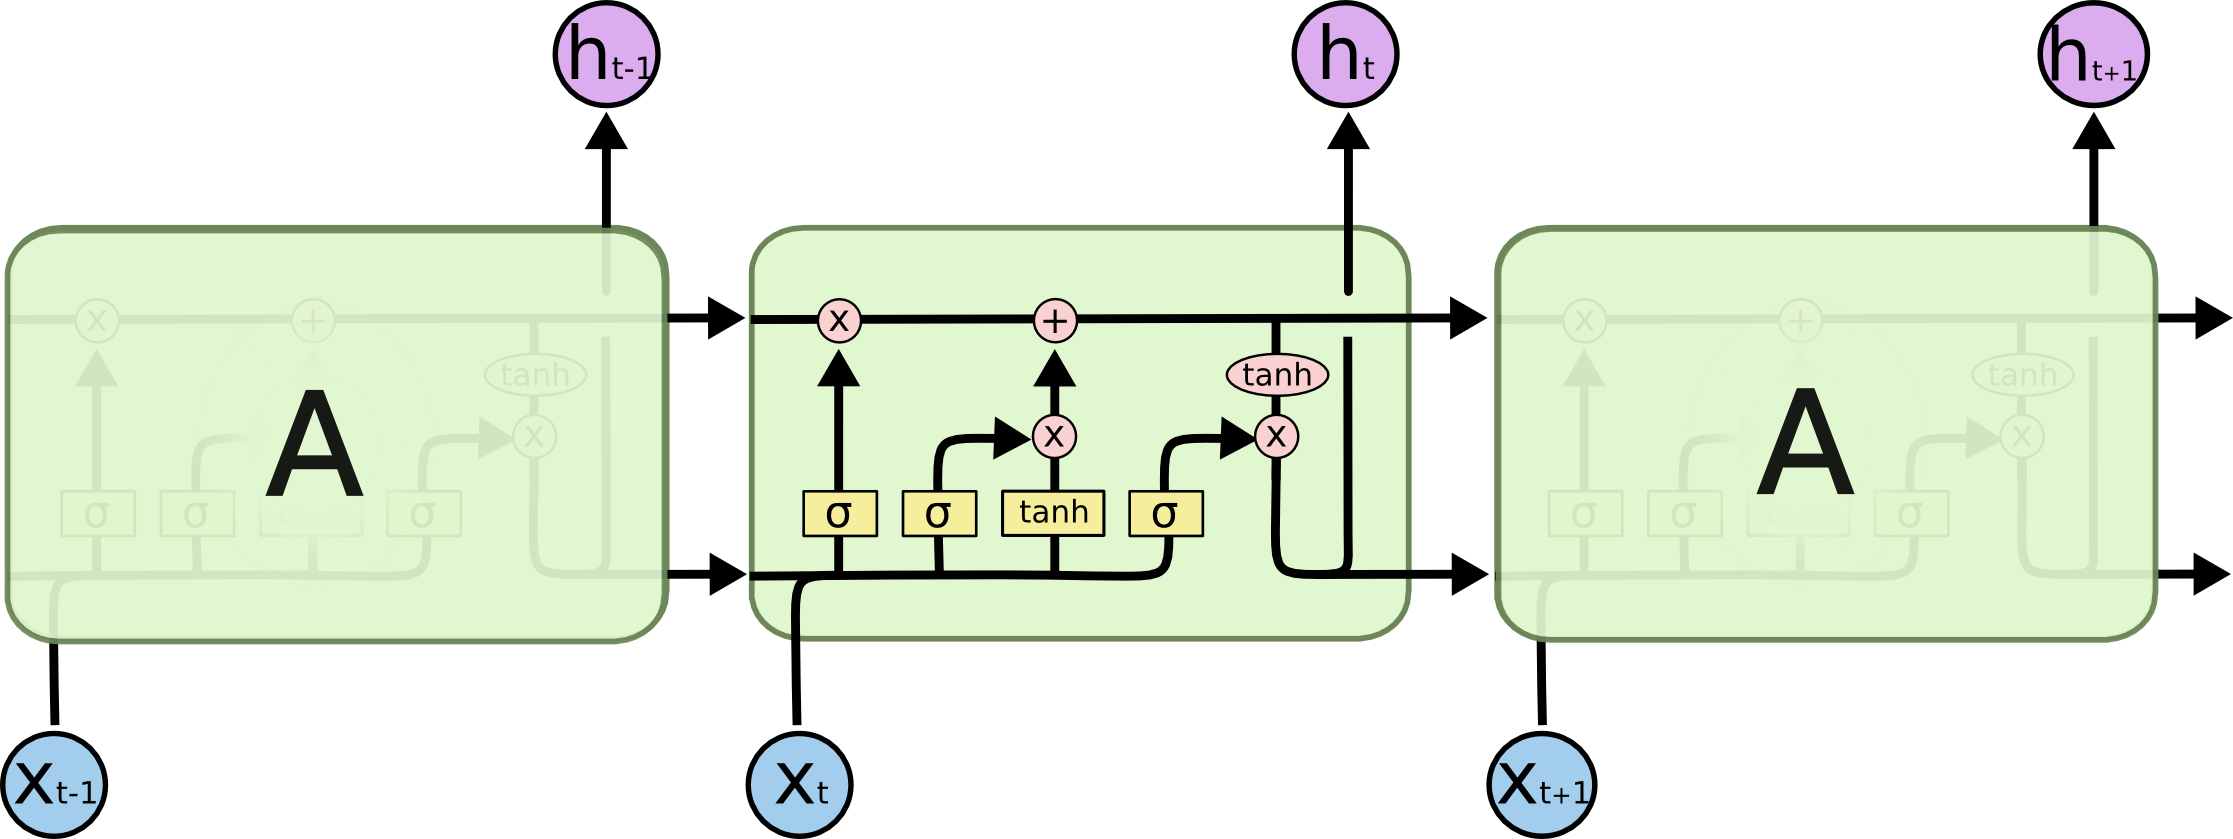
\includegraphics[width=\textwidth]{LSTM3-chain}
  \end{center}
\end{frame}



\begin{frame}{LSTM Formally}
  \begin{eqnarray*}
    R(\bold \bolds_{i-1}, \boldx_i) &=& [\boldc_i, \boldh_i]  \\
    \boldc_i &=& \boldj \odot \boldi  + \bold f \odot \bold c_{i-1}    \\
    \boldh_i &=& \tanh(\boldc_i) \odot \boldo\\ 
    \boldi &=& \tanh(\boldx \boldW^{xi} + \boldh_{i-1}\boldW^{hi} + \boldb^i) \\
    \boldj &=& \sigma(\boldx \boldW^{xj} + \boldh_{i-1}\boldW^{hj} + \boldb^j) \\
    \boldf &=& \sigma(\boldx \boldW^{xf} + \boldh_{i-1}\boldW^{hf} + \boldb^f) \\
    \boldo &=& \tanh(\boldx \boldW^{xo} + \boldh_{i-1}\boldW^{ho} + \boldb^o) \\
  \end{eqnarray*}
  \begin{itemize}
    \item (eeks.)
  \end{itemize}
  % \item $\boldf$; forget gate
  % \item $\boldi$; input gate
  % \item $\boldc$; cell state
  % \item $\boldh$; hidden state
  % \item $\boldo$; output gate (not very important)
  % \end{itemize}
\end{frame}

\begin{frame}{}
  \begin{center}
    \includegraphics[width=\textwidth]{good}
  \end{center}
\end{frame}

\begin{frame}{Unreasonable Effectiveness of RNNs}
  \url{http://karpathy.github.io/2015/05/21/rnn-effectiveness/}
\end{frame}

\begin{frame}
  \begin{center}
    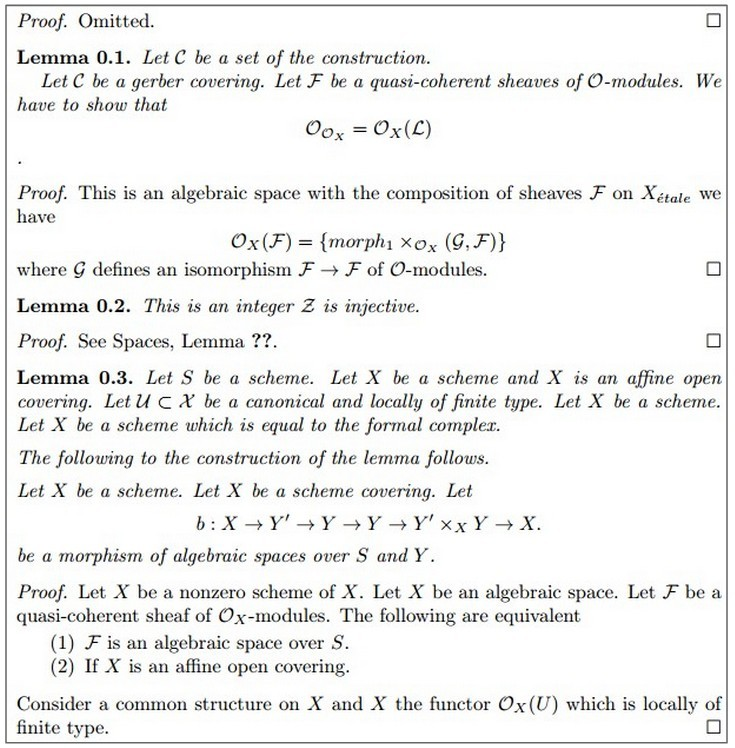
\includegraphics[width=0.8\linewidth]{../latex3}
  \end{center}
\end{frame}

\begin{frame}[fragile]
\begin{verbatim}
PANDARUS:
Alas, I think he shall be come approached and the day
When little srain would be attain'd into being never fed,
And who is but a chain and subjects of his death,
I should not sleep.

Second Senator:
They are away this miseries, produced upon my soul,
Breaking and strongly should be buried, when I perish
The earth and thoughts of many states.

DUKE VINCENTIO:
Well, your wit is in the care of side and that.
\end{verbatim}
\end{frame}

\begin{frame}{Music Composition}
  \url{http://www.hexahedria.com/2015/08/03/composing-music-with-recurrent-neural-networks/}
\end{frame}

\begin{frame}{Today's Lecture}
  \begin{itemize}
  \item Build up to LSTMs 
    \air 

  \item Note: Development is ahistoric, later papers first.
    \air

  \item Main idea: Getting around the vanishing gradient issue.   
  \end{itemize}
\end{frame}

\section{Highway Networks}

\begin{frame}{Review: Deep ReLU Networks}
  \[NN_{layer}(\boldx) = \relu(\boldx \boldW^1 + \boldb^1)  \]

  \begin{itemize}
  \item Given a input $\boldx$ can build arbitrarily deep fully-connected networks.
    \air 

  \item Deep Neural Network (DNN) : 
    \[NN_{layer}(NN_{layer}(NN_{layer}(\ldots NN_{layer}(\boldx))))\]
    \air 

  \end{itemize}
\end{frame}

\begin{frame}{Deep Networks}
  \[NN_{layer}(\boldx) = \relu(\boldx \boldW^1 + \boldb^1)  \]

      \begin{center}
      \scalebox{0.7}{\Tree [ .$\boldh_n$ [ .$\boldh_{n-1}$ [ .$\ldots$  [ .$\boldh_2$ [ .$\boldh_1$ $\boldx$ ] ] ]  ]  ] }
    \end{center}
    \pause
    
  \begin{itemize}
  \item  Can have similar issues with vanishing gradients.
  \end{itemize}
  \[ \frac{\partial L}{\partial h_{n-1,j_{n-1}} }   =  \sum_{j_n}  \indicator(h_{n, j_n} > 0) W_{j_{n-1},j_n}  \frac{\partial L}{\partial h_{n, j_n}}     \]

\end{frame}

\begin{frame}{Review: NLM Skip Connections}
  \begin{center}
    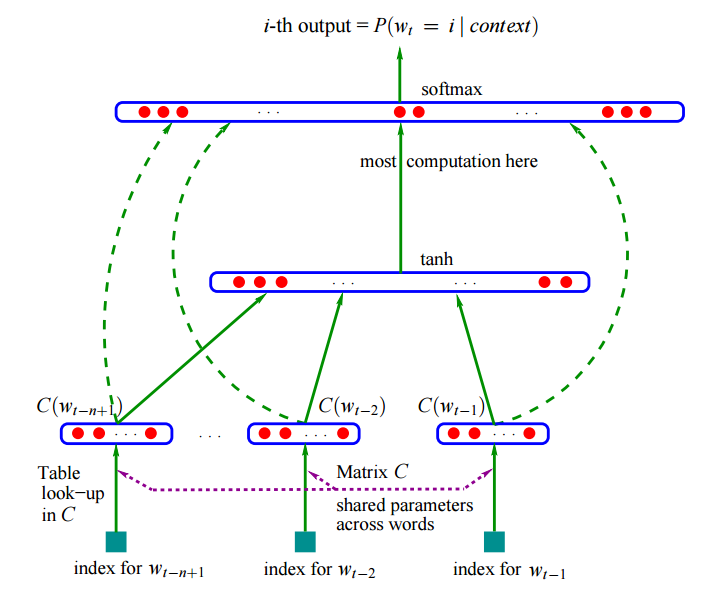
\includegraphics[width=7cm]{bengio}
  \end{center}
\end{frame}


\begin{frame}{Thought Experiment: Additive Skip-Connections}
  \[NN_{sl1}(\boldx) = \frac{1}{2} \relu(\boldx \boldW^1 + \boldb^1) + \frac{1}{2} \boldx \]
      \begin{center}
      \scalebox{0.7}{
        \begin{tikzpicture}
          \Tree [ .\node{$\boldh_n$}; [ .\node{$\boldh_{n-1}$}; [
          .$\ldots$ [ .\node(hc){$\boldh_3$}; [ .\node(hb){$\boldh_2$}; [
          .\node(ha){$\boldh_1$}; \node(x){$\boldx$}; ] ] ] ] ] ]
          \draw[dashed] (x) edge[bend left] (hb);
          \draw[dashed] (ha) edge[bend right] (hc);
        \end{tikzpicture}
      }
    \end{center}
  
\end{frame}

\begin{frame}{Exercise: Gradients}

  Exercise: What is the gradient of $\frac{\partial L}{\boldh_{n-1}}$ with skip-connections?
  Inductively what happens?

  \begin{center}
    \scalebox{0.7}{
      \begin{tikzpicture}
        \Tree [ .\node{$\boldh_n$}; [ .\node{$\boldh_{n-1}$}; [
        .$\ldots$ [ .\node(hc){$\boldh_3$}; [ .\node(hb){$\boldh_2$};
        [ .\node(ha){$\boldh_1$}; \node(x){$\boldx$}; ] ] ] ] ] ]
        \draw[dashed] (x) edge[bend left] (hb); \draw[dashed] (ha)
        edge[bend right] (hc);
      \end{tikzpicture}
    }
  \end{center}
\end{frame}


\begin{frame}{Exercise}
  We now have the average of two terms. One with no saturation condition or multiplicative term.
  \air 
  
  \begin{eqnarray*}
    \frac{\partial L}{\partial h_{n-1,j_{n-1}} }  =  &\frac{1}{2}& (\sum_{j_n}   \indicator(h_{n, j_n} > 0) W_{j_{n-1},j_n} \frac{\partial L}{\partial h_{n, j_n}}) + \\
    &\frac{1}{2}& ( h_{n-1, j_{n-1}} \frac{\partial L}{\partial h_{n, j_{n-1}}}) \\ 
  \end{eqnarray*}
\end{frame}

\begin{frame}{Thought Experiment 2: Dynamic Skip-Connections}
  \begin{eqnarray*}
    NN_{sl2}(\boldx) &=& (1-t) \relu(\boldx \boldW^1 + \boldb^1) + t \boldx \\
    t &=& \sigma(\boldx \boldW^t + b^t) \\
    \boldW^1 &\in& \reals^{\dhid \times \dhid} \\
    \boldW^t &\in& \reals^{\dhid \times 1} 
  \end{eqnarray*}


      \begin{center}
      \scalebox{0.7}{
        \begin{tikzpicture}
          \Tree [ .\node{$\boldh_n$}; [ .\node{$\boldh_{n-1}$}; [
          .$\ldots$ [ .\node(hc){$\boldh_3$}; [ .\node(hb){$\boldh_2$}; [
          .\node(ha){$\boldh_1$}; \node(x){$\boldx$}; ] ] ] ] ] ]
          \draw[dashed] (x) edge[bend left] (hb);
          \draw[dashed] (ha) edge[bend right] (hc);
        \end{tikzpicture}
      }
    \end{center}
\end{frame}


\begin{frame}{Dynamic Skip-Connections: intuition}
  \begin{eqnarray*}
    NN_{sl2}(\boldx) &=& (1-t) \relu(\boldx \boldW^1 + \boldb^1) + t \boldx \\
    t &=& \sigma(\boldx \boldW^t + b^t) \\
  \end{eqnarray*}

  \begin{itemize}
  \item No longer directly computing the next layer $\boldh_i$. 
    \air 

  \item Instead computing $\Delta \boldh$ and dynamic update proportion $t$.

    \air 
  \item Seems like a small change from DNN. Why does this matter?
  \end{itemize}
\end{frame}

\begin{frame}{Dynamic Skip-Connections Gradient}
  \begin{eqnarray*}
    NN_{sl2}(\boldx) &=& (1-t) \relu(\boldx \boldW^1 + \boldb^1) + t \boldx \\
    t &=& \sigma(\boldx \boldW^t + b^t) 
  \end{eqnarray*}
  \begin{itemize}
  \item The $t$ values are saved on the forward pass.
  \item $t$ allows for a direct flow of gradients to earlier layers. 
  \end{itemize}


  \begin{eqnarray*}
     \frac{\partial L}{\partial h_{n-1,j_{n-1}} }  =  &(1-t)& (\sum_{j_n}   \indicator(h_{n, j_n} > 0) W_{j_{n-1},j_n} \frac{\partial L}{\partial h_{n, j_n}}) \\
    + &t& ( h_{n-1, j_{n-1}} \frac{\partial L}{\partial h_{n, j_{n-1}}}) + \ldots \\ 
  \end{eqnarray*}

  \begin{itemize}
  \item (What is the $\ldots$?)
  \end{itemize}

\end{frame}



\begin{frame}{Dynamic Skip-Connections}
  \begin{eqnarray*}
    NN_{sl2}(\boldx) &=& (1-t) \relu(\boldx \boldW^1 + \boldb^1) + t \boldx \\
    t &=& \sigma(\boldx \boldW^t + b^t) 
  \end{eqnarray*}


  \begin{eqnarray*}
     \frac{\partial L}{\partial h_{n-1,j_{n-1}} }  =  &(1-t)& (\sum_{j_n}   \indicator(h_{n, j_n} > 0) W_{j_{n-1},j_n} \frac{\partial L}{\partial h_{n, j_n}}) \\
    + &t& ( h_{n-1, j_{n-1}} \frac{\partial L}{\partial h_{n, j_{n-1}}}) + \ldots \\ 
  \end{eqnarray*}

  \begin{itemize}
  \item Note: $\boldh$ and $\boldW^t$ are also receiving gradients through the sigmoid!
    \air
  \item (Backprop is fun.)
  \end{itemize}
\end{frame}

\begin{frame}{Highway Network (Srivastava et al., 2015)}
  \begin{itemize}
  \item Now add a combination at each dimension.
  \item $\odot$ is point-wise multiplication. 
  \end{itemize}
  \begin{eqnarray*}
    NN_{highway}(\boldx) &=& (1-\boldt) \odot \tilde{\boldh} + \boldt \odot \boldx \\
    \tilde{\boldh} &=& \relu(\boldx \boldW^1 + \boldb^1) \\
    \boldt &=& \sigma(\boldx \boldW^t + \boldb^t) \\
    \boldW^t, \boldW^1 &\in& \reals^{\dhid \times \dhid} \\
    \boldb^t, \boldb^1 &\in& \reals^{1 \times \dhid} 
  \end{eqnarray*}
  \begin{itemize}
  \item $\tilde{\boldh}$; \textit{transform} (e.g. standard MLP layer)
  \item $\boldt$; \textit{carry} (dimension-specific dynamic skipping)
  \end{itemize}
\end{frame}

\begin{frame}{Highway Gradients}
  \begin{itemize}
  \item The $\boldt$ values are saved on the forward pass.
    \air 
  \item $t_j$ determines the update of dimension $j$. 
  \end{itemize}
  \begin{eqnarray*}
     \frac{\partial L}{\partial h_{n-1,j_{n-1}} }  =  && (\sum_{j_n} (1-t_{j_n})  \indicator(h_{n, j_n} > 0) W_{j_{n-1},j_n} \frac{\partial L}{\partial h_{n, j_n}}) \\
    + &t_{j_{n-1}}& ( h_{n-1, j_{n-1}} \frac{\partial L}{\partial h_{n, j_{n-1}}}) + \ldots \\ 
  \end{eqnarray*}
\end{frame}


\begin{frame}{Intuition: Gating}
  \begin{itemize}
  \item This is known as the \textit{gating} operation
    \[ \boldt \odot \boldx \]
    \air 

  \item Allows vector $\boldt$ to mask or gate $\boldx$.
    \air

  \item True gating would have $\boldt \in \{0,1\}^{\dhid}$

    \air 
  \item Approximate with the sigmoid,
    \[\boldt = \sigma( \boldW^t \boldx + \boldb) \] 
  \end{itemize}
\end{frame}

\section{Gated Recurrent Unit (GRU)}

\begin{frame}{Back To Acceptor RNNs}
  \begin{itemize}

  \item Acceptor RNNs are deep networks with shared weights.

  \item Elman tanh layers 
    \[ NN(\boldx, \bolds) = \tanh( \bolds \boldW^s  +  \boldx \boldW^x  + \boldb).\]
    \air 
  \end{itemize}
  \begin{center}
    \vspace{-1cm}

    \begin{tikzpicture}
      \Tree [ .$\bolds_n$ [ .$\ldots$ [ .\node(sd){$\bolds_4$}; [
      .\node(sc){$\bolds_3$}; [ .\node(sb){$\bolds_2$}; [
      .\node(sa){$\bolds_1$}; \node(sz){$\bolds_0$}; $\boldx_1$ ]
      $\boldx_2$ ] $\boldx_3$ ] $\boldx_4$ ] $\ldots$ ] $\boldx_n$ ]
    \end{tikzpicture}
  \end{center}
\end{frame}


\begin{frame}{RNN with Skip-Connections}

  \begin{itemize}
    \item Can replace layer with modified highway layer. 
    \begin{eqnarray*}
      R(\bolds_{i-1}, \boldx_i) &=& (1-\boldt) \odot \tilde{\boldh} + \boldt \odot \bolds_{i-1} \\
      \tilde{\boldh} &=& \tanh(\boldx \boldW^x + \bolds_{i-1} \boldW^s + \boldb)  \\
      \boldt &=& \sigma(\boldx \boldW^{xt} + \bolds_{i-1}\boldW^{st} + \boldb^t) \\
      \boldW^{xt}, \boldW^{x} &\in& \reals^{\din \times \dhid} \\
      \boldW^{st}, \boldW^{s} &\in& \reals^{\dhid \times \dhid} \\
      \boldb^t, \boldb &\in& \reals^{1 \times \dhid} \\
    \end{eqnarray*}
  \end{itemize}

\end{frame}

\begin{frame}{RNN with Skip-Connections}
  \begin{center}
    \begin{tikzpicture}
      \Tree [ .$\bolds_n$ [ .$\ldots$ [ .\node(sd){$\bolds_4$}; [ .\node(sc){$\bolds_3$}; [ .\node(sb){$\bolds_2$}; [ .\node(sa){$\bolds_1$}; \node(sz){$\bolds_0$}; $\boldx_1$ ]
      $\boldx_2$ ] $\boldx_3$ ] $\boldx_4$ ] $\ldots$ ] $\boldx_n$ ];
      \draw (sz) edge[dashed, bend left] (sb);
      \draw (sa) edge[dashed, bend left] (sc);
      \draw (sb) edge[dashed, bend left] (sd);
    \end{tikzpicture}
  \end{center}
\end{frame}

\begin{frame}{Final Idea: Stopping flow}
  \begin{itemize}
  \item For many tasks, it is useful to halt propagation.
    \air
  \item Can do this by applying a reset gate $\boldr$. 
    \air 

    \begin{eqnarray*}
      \tilde{\boldh} &=& \tanh(\boldx \boldW^x + (\boldr \odot \bolds_{i-1})  \boldW^s + \boldb)  \\
      \boldr &=& \sigma(\boldx \boldW^{xr} + \bolds_{i-1}\boldW^{sr} + \boldb^r) \\
    \end{eqnarray*}

    
  \end{itemize}
\end{frame}


\begin{frame}{Gated Recurrent Unit (GRU) (Cho et al 2014)}
    \begin{eqnarray*}
      R(\bolds_{i-1}, \boldx_i) &=& (1-\boldt) \odot \tilde{\boldh} + \boldt \odot \bolds_{i-1} \\
      \tilde{\boldh} &=& \tanh(\boldx \boldW^x + (\boldr \odot \bolds_{i-1})  \boldW^s + \boldb)  \\
      \boldr &=& \sigma(\boldx \boldW^{xr} + \bolds_{i-1}\boldW^{sr} + \boldb^r) \\
      \boldt &=& \sigma(\boldx \boldW^{xt} + \bolds_{i-1}\boldW^{st} + \boldb^t) \\
      \boldW^{xt}, \boldW^{xr}, \boldW^{x} &\in& \reals^{\din \times \dhid} \\
      \boldW^{st}, \boldW^{sr}, \boldW^{s} &\in& \reals^{\dhid \times \dhid} \\
      \boldb^t, \boldb &\in& \reals^{1 \times \dhid} \\
    \end{eqnarray*}

    \begin{itemize}
    \item $\boldt$; dynamic skip-connections
    \item $\boldr$; reset gating
    \item $\bolds$; hidden state
    \item $\tilde{\boldh}$; gated MLP
    \end{itemize}
\end{frame}

\begin{frame}{Example: Language Modeling}
  \begin{itemize}
  \item In non-Markovian language modeling, treat corpus as a sequence
    \air 
  \item $\boldr$ allows resetting the state after a sequence. 
  \end{itemize}
  \begin{quote}
    consumers may want to move their telephones a little closer to the
    tv set $<$/s$>$ $<$unk$>$ $<$unk$>$ watching abc 's monday night
    football can now vote during $<$unk$>$ for the greatest play in N
    years from among four or five $<$unk$>$ $<$unk$>$ $<$/s$>$ two
    weeks ago viewers of several nbc $<$unk$>$ consumer segments
    started calling a N number for advice on various $<$unk$>$ issues
    $<$/s$>$ and the new syndicated reality show hard copy records
    viewers ' opinions for possible airing on the next day 's show
    $<$/s$>$
  \end{quote}
\end{frame}


\section{LSTM}

\begin{frame}{LSTM}
  \begin{itemize}
  \item Long Short-Term Memory network uses the same idea. 
    \air 

  \item Model has three gates, input, output, forget. 
    \air 

  \item Developed first, but a bit harder to follow. 
    \air 

  \item Seems to be better at LM, comparable to GRU on other tasks.
  \end{itemize}
\end{frame}

\begin{frame}{LSTMs State}

  The state $\bolds_i$ is made of 2 components :
  \begin{itemize}
  \item $\boldc_i$; cell
  \item $\boldh_i$; hidden
  \end{itemize}

    \begin{eqnarray*}
      R(\bolds_{i-1}, \boldx_i) &=& [\boldc_i, \boldh_i]  \\
      % \alert{\boldh_i} &=& \tanh(\boldc_i) \\ 
      % \boldc_i &=& (1-\boldt) \odot \tilde{\boldh}  + \boldt \odot \bold c_{i-1}    \\
      % \tilde{\boldh} &=& \tanh(\boldx \boldW^{xi} + \boldh_{i-1}\boldW^{hi} + \boldb^i) \\
      % \boldt &=& \sigma(\boldx \boldW^{xt} + \boldh_{i-1}\boldW^{ht} + \boldb^t) \\
    \end{eqnarray*}

\end{frame}

\begin{frame}{LSTM Development: Input and Forget Gates}
  The cell is updated with $\Delta \boldc$, not a convex combination (two gates). 

    \begin{eqnarray*}
      R(\bolds_{i-1}, \boldx_i) &=& [\boldc_i, \boldh_i]  \\
      \boldc_i &=& \alert{\boldj \odot \tilde{\boldh}  + \boldf \odot \bold c_{i-1} } \\
      \tilde{\boldh} &=& \tanh(\boldx \boldW^{xi} + \boldh_{i-1}\boldW^{hi} + \boldb^i) \\
      \boldj &=& \sigma(\boldx \boldW^{xj} + \boldh_{i-1}\boldW^{hj} + \boldb^j) \\
      \boldf &=& \sigma(\boldx \boldW^{xf} + \boldh_{i-1}\boldW^{hf} + \boldb^f) 
    \end{eqnarray*}

    \begin{itemize}
    \item $\boldc_i$; cell
    \item $\boldj$; input gate
    \item $\boldf$; forget gate
    \end{itemize}
\end{frame}


\begin{frame}{LSTM Development: Hidden}
  Hidden $\boldh_i$ squashes $\boldc_i$

    \begin{eqnarray*}
      R(\boldc_{i-1}, \boldx_i) &=& [\boldc_i, \boldh_i]  \\
      \alert{\boldh_i} &=& \tanh(\boldc_i) \\ 
      \boldc_i &=& \boldj \odot \tilde{\boldh}  + \boldf \odot \bold c_{i-1}  \\
      \tilde{\boldh} &=& \tanh(\boldx \boldW^{xi} + \boldh_{i-1}\boldW^{hi} + \boldb^i) \\
      \boldj &=& \sigma(\boldx \boldW^{xj} + \boldh_{i-1}\boldW^{hj} + \boldb^j) \\
      \boldf &=& \sigma(\boldx \boldW^{xf} + \boldh_{i-1}\boldW^{hf} + \boldb^f) 
    \end{eqnarray*}

    \begin{itemize}
    \item $\boldc_i$; cell
    \item $\boldh_i$; hidden
    \item $\boldj$; input gate
    \item $\boldf$; forget gate
    \end{itemize}
\end{frame}

% \begin{frame}{Long Short-Term Memory (without output)}
%     \begin{eqnarray*}
%       R(\bold \bolds_{i-1}, \boldx_i) &=& [\boldc_i, \boldh_i]  \\
%       \boldc_i &=& \boldj \odot \boldi  + \bold f \odot \bold c_{i-1}    \\
%       \boldh_i = \tanh(\boldc_i) %\odot \boldo
%       \boldi &=& \tanh(\boldx \boldW^{xi} + \boldh_{i-1}\boldW^{hi} + \boldb^i) \\
%       \boldj &=& \sigma(\boldx \boldW^{xj} + \boldh_{i-1}\boldW^{hj} + \boldb^j) \\
%       \boldf &=& \sigma(\boldx \boldW^{xf} + \boldh_{i-1}\boldW^{hf} + \boldb^f) \\
%       % \boldo &=& \tanh(\boldx \boldW^{xo} + \boldh_{i-1}\boldW^{ho} + \boldb^o) \\
%     \end{eqnarray*}
%     \begin{itemize}
%     \item $\boldf$; forget gate
%     \item $\boldi$; input gate
%     \item $\boldo$; output gate
%     \item $\boldc$; cell state
%     \item $\boldh$; hidden state
%     \end{itemize}
% \end{frame}


\begin{frame}{Long Short-Term Memory}
  Finally, another output gate is applied to $\boldh$
    \begin{eqnarray*}
      R(\bold \bolds_{i-1}, \boldx_i) &=& [\boldc_i, \boldh_i]  \\
      \boldc_i &=& \boldj \odot \boldi  + \bold f \odot \bold c_{i-1}    \\
      \boldh_i &=& \tanh(\boldc_i) \alert{\odot \boldo}\\ 
      \boldi &=& \tanh(\boldx \boldW^{xi} + \boldh_{i-1}\boldW^{hi} + \boldb^i) \\
      \boldj &=& \sigma(\boldx \boldW^{xj} + \boldh_{i-1}\boldW^{hj} + \boldb^j) \\
      \boldf &=& \sigma(\boldx \boldW^{xf} + \boldh_{i-1}\boldW^{hf} + \boldb^f) \\
      \boldo &=& \tanh(\boldx \boldW^{xo} + \boldh_{i-1}\boldW^{ho} + \boldb^o) \\
    \end{eqnarray*}
\end{frame}

\begin{frame}{Output Gate?}
  \begin{itemize}
  \item The output gate feels the most ad-hoc (why tanh?)
    \air 

  \item Luckily Jozefowicz et al (2015) find output not too important.
  \end{itemize}
\end{frame}

\begin{frame}
  \begin{center}
    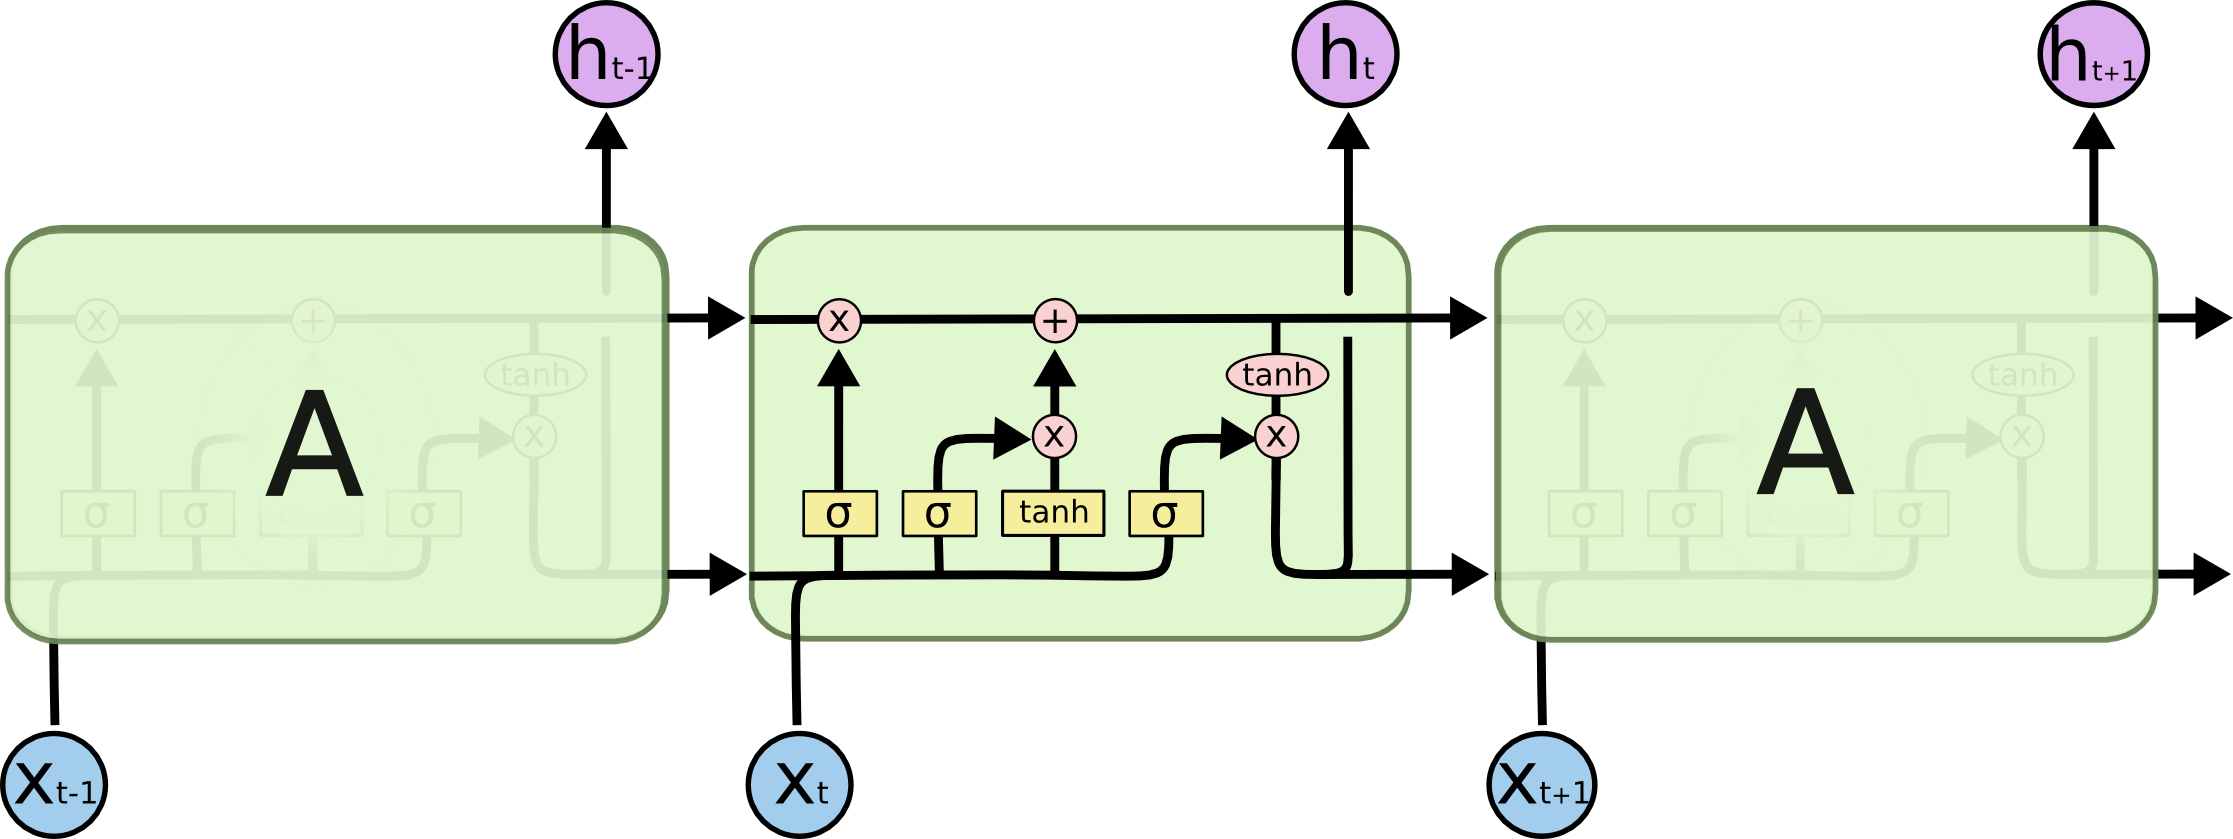
\includegraphics[width=\textwidth]{LSTM3-chain}
  \end{center}

\end{frame}

\begin{frame}{Accuracy Results (Jozefowicz et al, 2015) }
  \begin{center}
    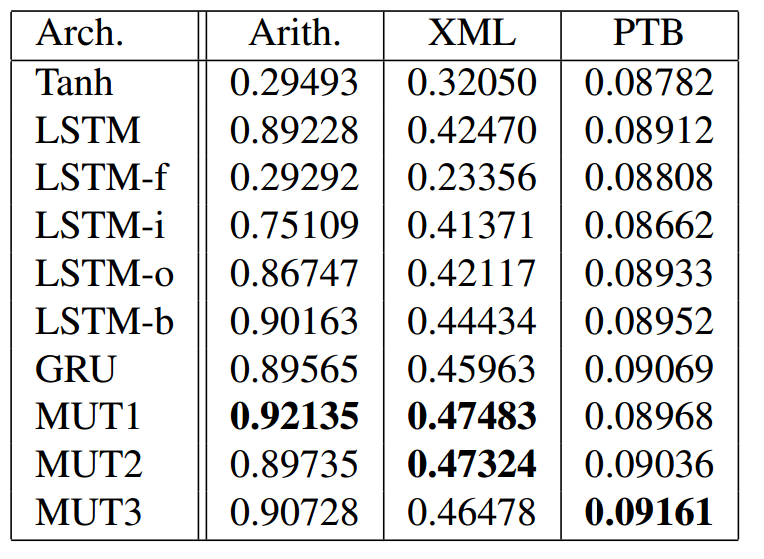
\includegraphics[width=8cm]{lstm-accuracy}
  \end{center}
  Accuracy of RNN models on three different tasks. LSTM models 
  include versions without the forget, input, and output gates. 
\end{frame}

\begin{frame}{English LM Results (Jozefowicz et al, 2015) }
  \begin{center}
    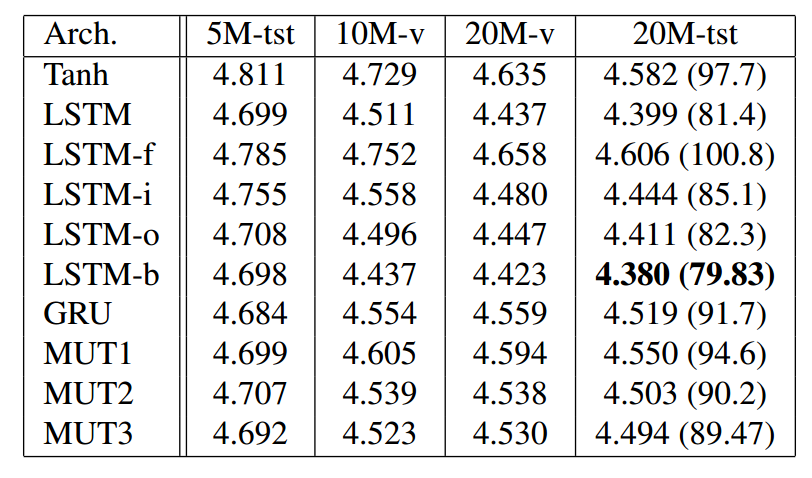
\includegraphics[width=10cm]{lstm-results}
  \end{center}
  \begin{center}
    NLL (Perplexity)
  \end{center}
\end{frame}




\end{document}
